% Modern editorial, markup and figure/layout contributions: CC-BY-SA-4.0.
% Historical text and illustrations: Leonhard Euler (1744), public domain.
% Component scope and upstream attribution: see RIGHTS.md.
% Vector redraw: Tabula I, Fig. 3. n and v are distinct points on one ordinate.
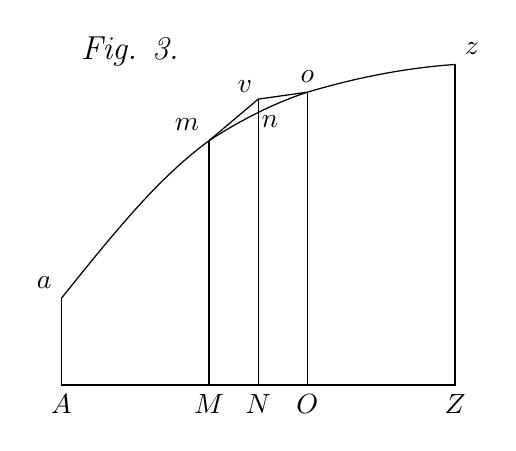
\begin{tikzpicture}[x=1.25cm,y=1.1cm,line width=.45pt]
\draw (0,1)--(0,0)--(4,0)--(4,3.7);
\draw (0,1) .. controls (.6,1.85) and (1,2.4) .. (1.5,2.82)
 .. controls (1.85,3.08) and (2.2,3.27) .. (2.5,3.38)
 .. controls (3,3.55) and (3.5,3.66) .. (4,3.7);
\draw (1.5,0)--(1.5,2.82) (2,0)--(2,3.30) (2.5,0)--(2.5,3.38);
\draw (1.5,2.82)--(2,3.30)--(2.5,3.38);
\foreach \x/\t in {0/A,1.5/M,2/N,2.5/O,4/Z}{\node[below] at (\x,0) {$\t$};}
\node[above left] at (0,1) {$a$};\node[above left] at (1.5,2.82) {$m$};
\node[below right,inner sep=1pt] at (2,3.15) {$n$};
\node[above left,inner sep=2pt] at (2,3.30) {$v$};
\node[above] at (2.5,3.38) {$o$};\node[above right] at (4,3.7) {$z$};
\node[anchor=west] at (.1,3.85) {\large\textit{Fig. 3.}};
\end{tikzpicture}
